\chapter*{Comparaisons des trois approches}

\section{Résumé}
Afin de résumer et de visualiser les comparaisons entre les trois approches, le tableau récapitulatif suivant est proposé(accompagné de son graphe) : 
\begin{table}[H]
	\centering
		\begin{tabular}{|c|c|}
			\hline
			\textbf{Approche}   & \textbf{Taux moy.} \\ \hline
			A*                  & 97,262\%           \\ \hline
			ACS                 & 99,908\%           \\ \hline
			AS                  & 99,615\%           \\ \hline
			\rowcolor[HTML]{FD6864} 
			BFS                 & 42,902\%           \\ \hline
			BSO                 & 99,914\%           \\ \hline
			Coût uniforme       & 93,215\%           \\ \hline
			DBSO                & 99,969\%           \\ \hline
			\rowcolor[HTML]{9AFF99} 
			DBSO parallèle      & 100,000\%          \\ \hline
			DFS                 & 93,268\%           \\ \hline
			Recherche gloutonne & 96,600\%           \\ \hline
		\end{tabular}%
	\caption{Récapitulatif de toutes les approches}
	\label{my-label}
\end{table}

\begin{figure}[H]
	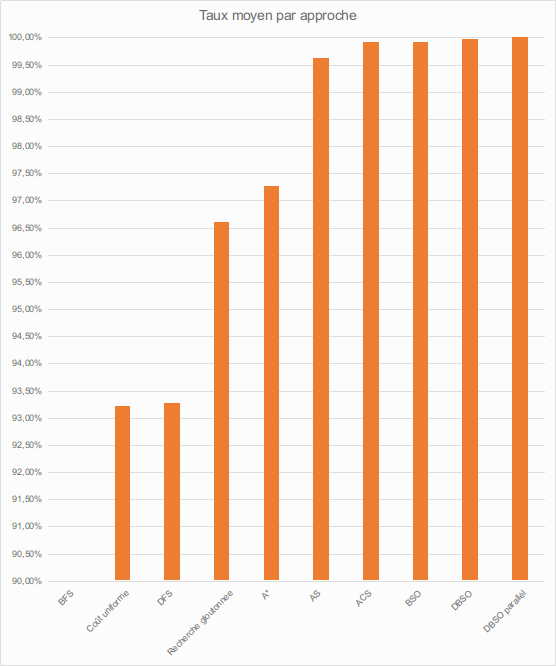
\includegraphics[width=\textwidth]{images/battleRoyale.png}
\end{figure}


\paragraph{Commentaires : }
Une vite observations peut être faite, c'est que les méthode de l'approche de la partie \ref{part1} sont très en dessous de la norme désirée, à titre d'exemple \textbf{BFS} n'atteint même pas la barre des 50\%, la meilleure méthode étant la modification dynamique de BSO que nous avons appelé \textbf{D-BSO}(Dynamic Bee Swarm Optimization) avec traitement parallèle dont le taux \textbf{MOYEN} de satisfaction est égale à 100\%.
